
%(BEGIN_QUESTION)
% Copyright 2010, Tony R. Kuphaldt, released under the Creative Commons Attribution License (v 1.0)
% This means you may do almost anything with this work of mine, so long as you give me proper credit

Two pressure switches are used in this burner management system (BMS) to ensure automatic shutoff of fuel gas to the burner in the event the gas pressure either falls below the low-pressure trip point, or exceeds the high-pressure trip point:

$$\includegraphics[width=15.5cm]{i04747x01.eps}$$

These switches are connected to the burner control relay as shown in this schematic diagram:

$$\includegraphics[width=15.5cm]{i04747x02.eps}$$

Suppose you needed to physically remove the low-pressure switch from the system to recalibrate it back in the instrument shop, but needed to keep the burner system operating as you did so.  Explain how you could ``fool'' the control circuit to allow removal of the PSL yet not disable all the other functions (Start, Stop, PSH shutdown).  Feel free to sketch over the schematic diagram to illustrate what you would do to the circuit.

\underbar{file i04747}
%(END_QUESTION)





%(BEGIN_ANSWER)

{\it Full credit for this answer:}

$$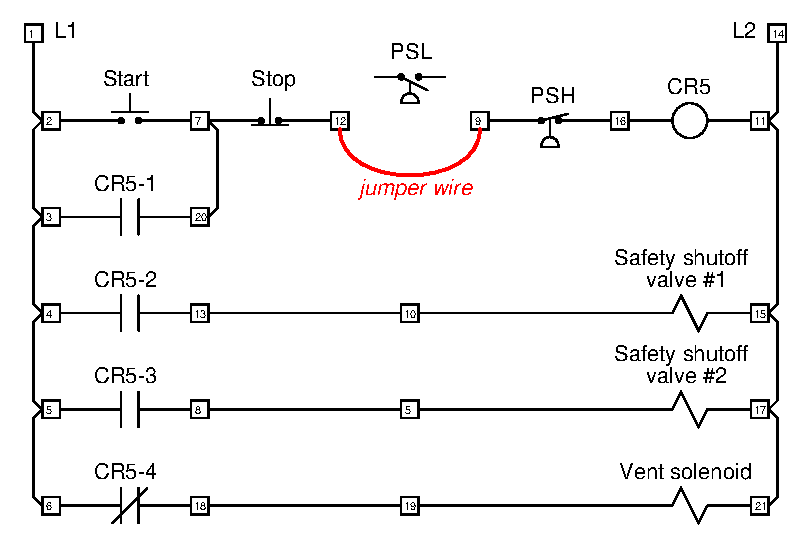
\includegraphics[width=15.5cm]{i04747x03.eps}$$

{\it Half credit for an answer that bypasses the missing PSL but also bypasses other functions (e.g. Stop button, PSH, etc.).}

%(END_ANSWER)





%(BEGIN_NOTES)

{\bf This question is intended for exams only and not worksheets!}

%(END_NOTES)


